\documentclass[UTF8,a4paper]{article}
\usepackage{ctex}
\usepackage{graphicx}
\graphicspath{{image/}}
\title{线性回归}
\author{Luke}
\begin{document}
\maketitle

\section{最小二乘}

对于$y=b+w\cdot x_{cp}$,定义损失函数(Loss function)来度量函数的好坏:

\begin{equation}
L(f)=L(w,b)=\sum^{10}_{n=1}(\hat{y}^n-(b+w\cdot x^{n}_{cp}))^2
\end{equation}

角标n表示第n个数据点。可以预见,当L取最小值时的函数$f$就是最好的函数,因此对L求导:

\begin{equation}
\frac{\partial}{\partial w}L=\sum^{10}_{n=1}2(\hat{y}^n-(b+w\cdot x^{n}_{cp}))x^{n}_{cp}=0
\end{equation}
\begin{equation}
\frac{\partial}{\partial b}L=\sum^{10}_{n=1}2(\hat{y}^n-(b+w\cdot x^{n}_{cp}))=0
\end{equation}

代入数据即可求出一组w和b的值。

\section{梯度下降}

任意取一$L(w_0,b_0)$,计算
\[\frac{\partial L}{\partial b}\mid _{w=w_0,b=b_0},\frac{\partial L}{\partial w}\mid _{w=w_0,b=b_0}\]
而
\[(-\eta\frac{\partial L}{\partial b},-\eta\frac{\partial L}{\partial w})\]
的方向就是L下降最快的方向。取
\[b_1=b_0-\eta\frac{\partial L}{\partial b}\]
\[w_1=w_0-\eta\frac{\partial L}{\partial w}\]
在$L(w_1,b_1)$重复此过程。($\eta$是选定的步长)

\section{欠拟合和过拟合}

对于同样的100组数据,选择多项式拟合的阶数较少会造成欠拟合,阶数较多会造成过拟合。欠拟合表现为拟合的模型偏差较大 (large bias) 但是方差较小 (small variance) ,过拟合表现为拟合的模型偏差较小 (small bias) 但是方差较大 (large variance) 。此处的偏差与方差描述不同训练数据得出的模型的集合与理想模型(图中的靶心)的对比。
\begin{figure}[ht]
\centering
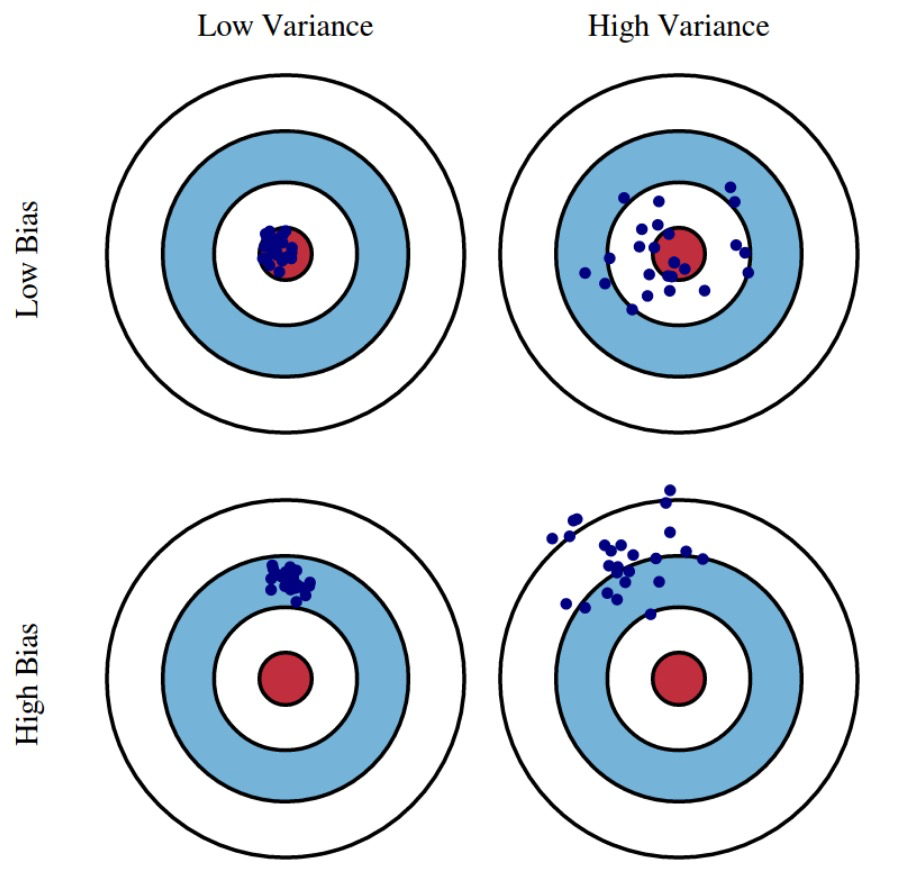
\includegraphics[width=300pt]{bias-variance.png}
\caption{bias和variance的示意图}
\label{bias-variance}
\end{figure}

通过增加数据的方法可以解决variance过大的问题,而在没有更多数据的时候,可以用regularzation(正则化)的方法减小variance,但是可能会同时增大bias.实际操作中需要选择恰当的模型来平衡两种误差使得总误差最小。

选择模型时要避免使用训练数据得出的几个模型,再用测试数据挑出最好的一个,这样会使真正应用场景下结果的不可控(图2),即图中真实数据的误差是大于0.5的。

\newpage

\begin{figure}[ht]
\centering
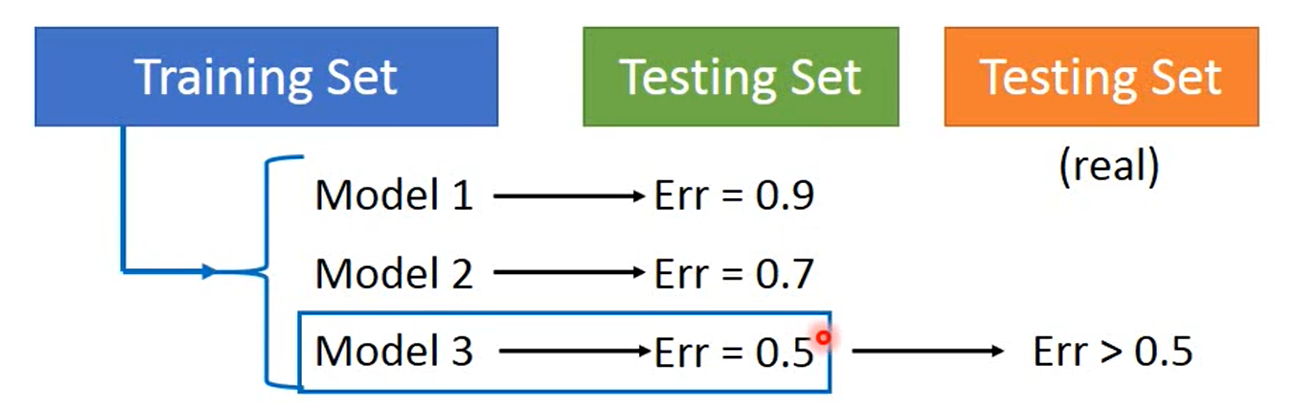
\includegraphics[width=300pt]{notdo.png}
\caption{不要采用这种方法}
\label{notdo}
\end{figure}

可以采用交叉验证(Cross Validation)的方法来避免这种情况,如图3将 training set 分为两部分,一部分作为 training set ,一部分作为 validation set ,通过验算 validation set 的 error 来决定选择哪个 model. 此时,不应再用 testing set 中的数据来返回验算其他 model ,这会将 testing set 变成一个新的 validation set ,从而影响模型的最终效果。
\begin{figure}[ht]
\centering
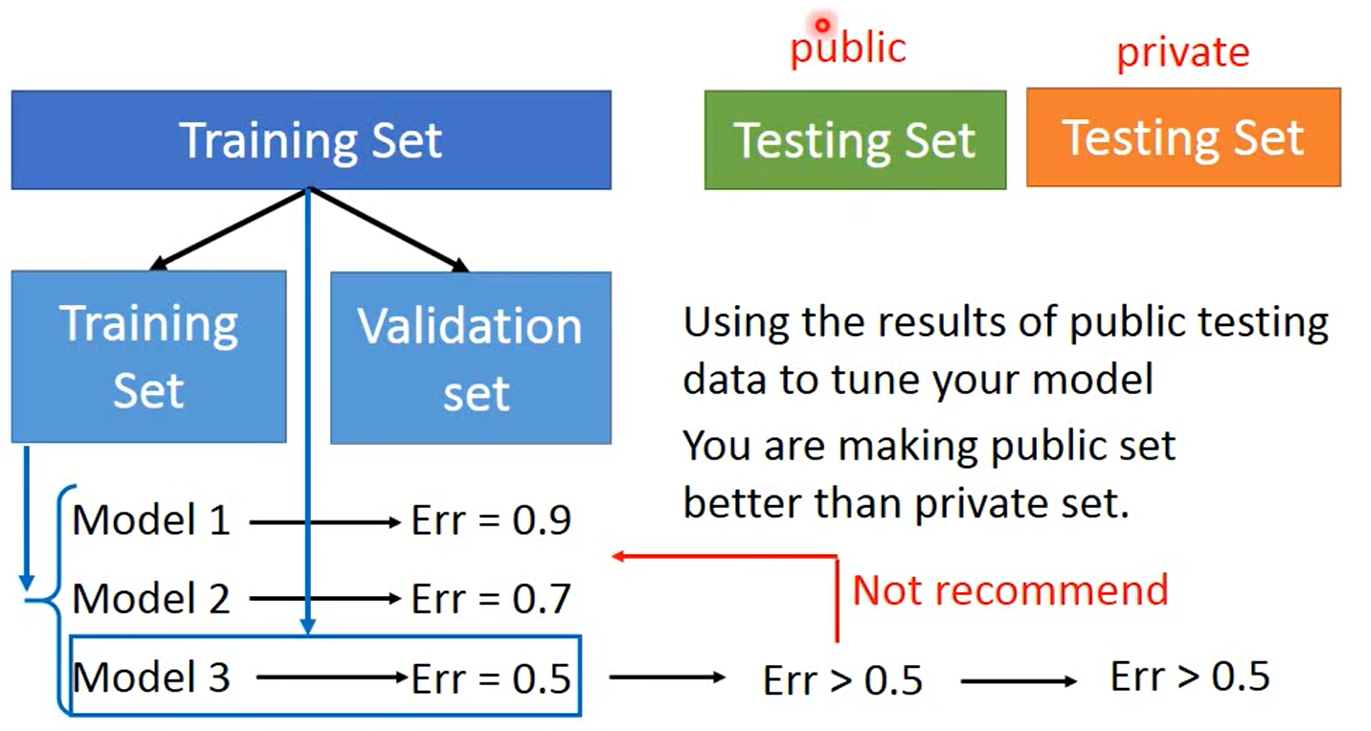
\includegraphics[width=300pt]{rec1.png}
\caption{可以采用这种方法}
\label{recommended1}
\end{figure}

在实际操作中这种方法会遇到如何分开 training set 的问题,这时可以使用 N-fold Cross Validation 的方法来避免可能出现的小概率事件(图4)。将 training set 分为三部分,分别作为训练集和测试集得出 error ,取平均 error 最小的 model 用 testing set 验算。

\newpage
\begin{figure}[ht]
\centering
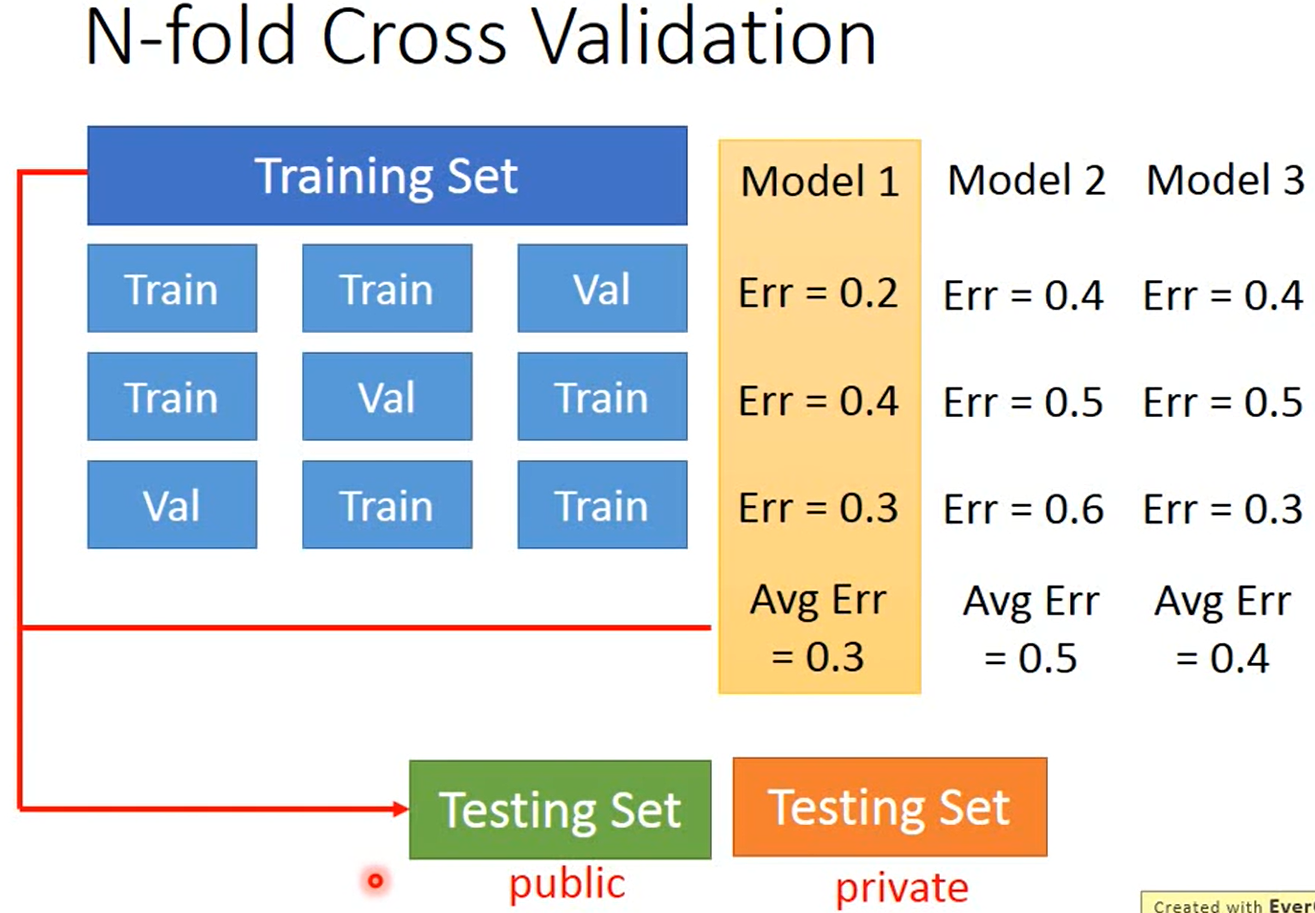
\includegraphics[width=300pt]{rec2.png}
\caption{可以采用这种方法}
\label{recommended2}
\end{figure}

\end{document}